\section{Setup it up}
\label{sec:setup}

To set up a project start Xcode and create a new project with an iOS Template. If this is your first attemp at programming an app, we suggest to start with a ``\textit{Single View Application}''. The ``\textit{Device Family}'' is up to you. The framework supports iPad, iPhone and to test your app without a hardware device, the simulator. 

In Xcode, your project has a file tree on the left. One of its folders is titled ``\textit{Frameworks}''. Drag the ``\textit{hamcast.framework}'' from your file manager onto that folder. It is not necessary to copy the framework into your project. You can use the options as seen in Figure \ref{fig:import}. Do the same for ``\textit{boost.framework}''.

\includeimage{pictures/import}{Import the the hamcast framework into your project.}{fig:import}

%\begin{figure}[h]
%	\centering
%  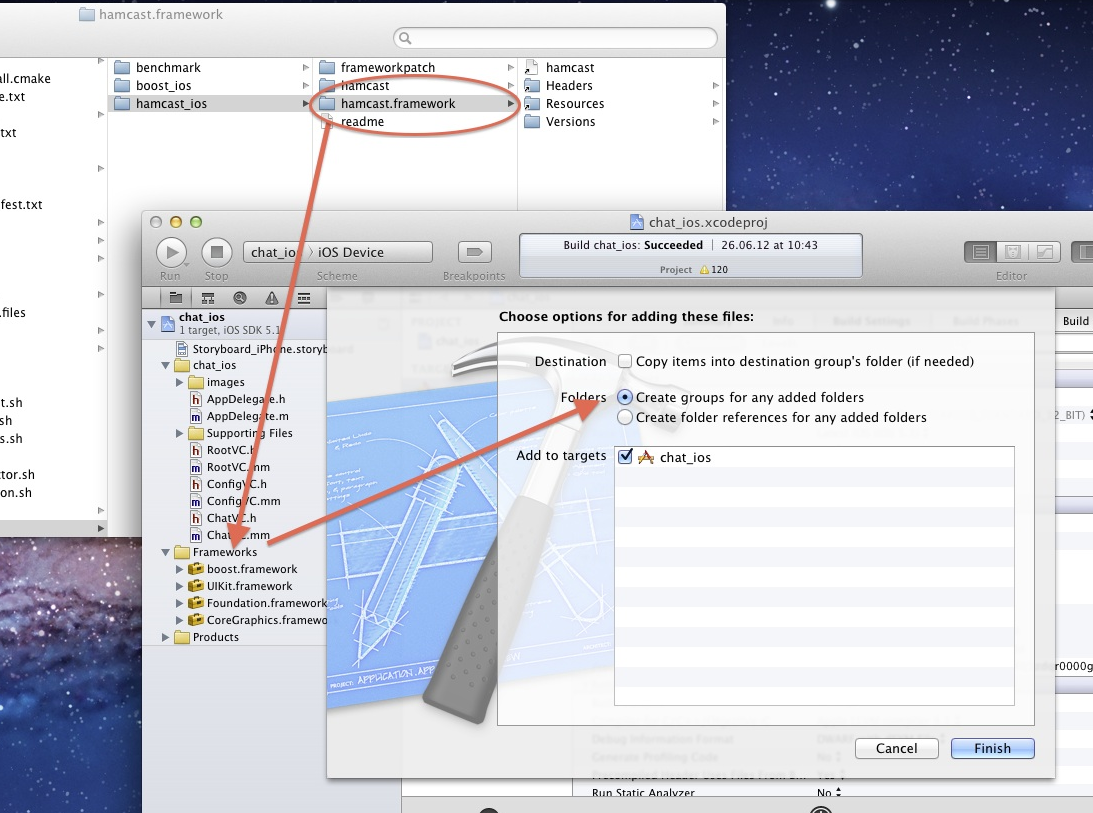
\includegraphics[width=1.0\textwidth]{pictures/import}
%	\caption{Import the the hamcast framework into your project.}
%	\label{fig:import}
%\end{figure}
